% !TeX spellcheck = fr_FR
\documentclass[a4paper]{report}


%% Language and font encodings
\usepackage[french]{babel}
\usepackage[utf8]{inputenc}
\usepackage[T1]{fontenc}

%% Sets page size and margins
\usepackage[a4paper,top=3cm,bottom=2cm,left=3cm,right=3cm,marginparwidth=1.75cm]{geometry}

%% Useful packages
\usepackage{biblatex}
\bibliography{report.bib}
\usepackage{graphicx}
\usepackage[colorinlistoftodos]{todonotes}
\usepackage{amsmath,amsthm,amssymb}
\usepackage[colorlinks=true, allcolors=blue]{hyperref}
\usepackage{listings}
\usepackage{color}
\usepackage{titlesec}
\definecolor{dkgreen}{rgb}{0,0.6,0}
\usepackage{textcomp}
\lstset{frame=tb,
  language=Python,
  aboveskip=3mm,
  belowskip=3mm,
  showstringspaces=false,
  columns=flexible,
  basicstyle={\ttfamily},
  numbers=none,
  numberstyle=\color{gray},
  keywordstyle=\color{blue},
  commentstyle=\color{dkgreen},
  stringstyle=\color{dkgreen},
  breaklines=true,
  breakatwhitespace=true,
  tabsize=2
}
\setlength{\parskip}{1em}

\titleformat{\chapter}{\normalfont\huge}{\bf\thechapter}{12pt}{\huge\bf}

\title{TB - Gleam}

\author{Antoine Friant}
\begin{document}
\pagenumbering{roman}
\begin{titlepage}

\newcommand{\HRule}{\rule{\linewidth}{0.5mm}} % Defines a new command for the horizontal lines, change thickness here
%----------------------------------------------------------------------------------------
%	LOGO SECTION
%----------------------------------------------------------------------------------------


\includegraphics[width=2in]{img/logoheig.png}\\ % Include a department/university logo - this will require the graphicx package

\vspace{1in}

\center % Center everything on the page
 
%----------------------------------------------------------------------------------------
%	HEADING SECTIONS
%----------------------------------------------------------------------------------------

\textsc{\LARGE HEIG-VD}\\[1.5cm] % Name of your university/college
\textsc{\Large Rapport intermédiaire}\\[0.5cm] % Major heading such as course name

%----------------------------------------------------------------------------------------
%	TITLE SECTION
%----------------------------------------------------------------------------------------

\HRule \\[0.4cm]
{ \huge \bfseries La Terre de nuit vue de l'espace }\\ % Title of your document
\Large\HRule \\[2cm]
\normalsize
%----------------------------------------------------------------------------------------
%	AUTHOR SECTION
%----------------------------------------------------------------------------------------

\begin{minipage}[t]{0.48\textwidth}
\begin{flushleft} \large
Antoine \textsc{Friant} \\
\normalsize
Haute École d'Ingénierie et de Gestion du Canton de Vaud\\
Yverdon-les-Bains, VD, CH
\texttt{antoine.friant@gmail.com}
\end{flushleft}
\end{minipage}
~
\begin{minipage}[t]{0.49\textwidth}
\begin{flushright} \large
% empty page for alignement
\end{flushright}
\end{minipage}\\[2cm]



{\large \today}\\
 

\vfill % Fill the rest of the page with whitespace

\end{titlepage}

\chapter{Cahier des charges}

\section{Résumé du problème}
Les données géographiques sont nécessaires pour la prise de décisions importantes. Cependant la fiabilité et la disponibilité de ces données ne sont pas homogènes dans le temps et selon le lieu. Certaines de ces données ont une forte corrélation avec la lumière perçue par les satellites pendant la nuit.

Grâce à l'apprentissage automatique (\textit{machine learning}), il est possible d'entraîner un réseau de neurones sur des données d'une date et d'un lieu connus pour reconstituer une carte de données géographiques à partir d'une image satellite nocturne.

Le travail à effectuer consiste à explorer différents types de données géographiques afin d'en choisir un, et faire de la prédiction sur ce type de données grâce à un réseau de neurones.

\section{Objectifs}
Le TB consiste dans un premier temps à explorer les données suivantes :

\begin{itemize}
\item Images satellites noctures de la Terre,
\item Population humaine,
\item Population animale,
\item Densité végétale,
\item PIB,
\end{itemize}

Et toutes autres données jugées pertinentes dans le but d'entraîner un réseau de neurones capable de prédire une estimation d'une donnée utile, à partir d'une image satellite de la terre de nuit.

La réalisation d'une application qui entraîne et exploite ce réseau de neurones est l'objectif de la seconde partie du TB.

Le but final est de pouvoir estimer, grâce au machine learning, des informations dont on ne possède pas de données à jour. Et cela à partir d'images satellites de nuit récentes, ou d'une combinaisons de ces images avec une autre donnée à jour.

\section{Limitations}
L'application sera compatible avec Windows 10 et Archlinux, et nécessitera l'installation de librairies tierces (telles que Keras et TensorFlow).
Elle ne possèdera pas nécessairement d'interface utilisateur.

L'utilisateur sera responsable de fournir les données à l'application dans un format supporté.

\section{Description fonctionnelle}
L'application prend en argument au moins deux jeux de données géographiques de format imposé : une image satellite nocturne et un autre type de donnée à déterminer au cours du projet. Après un long temps d'entraînement (une semaine au maximum, dépend de la machine utilisée), un modèle est généré.

Une fois le modèle généré, il est sauvegardé et réutilisable sur une autre image satellite nocturne (d'une date et/ou d'une région différente). Lorsque le modèle est appliqué sur une image satellite, une carte est recréée, affichant le résultats des prédictions.

Par exemple, si au cours du travail de bachelor il s'avère que la population par kilomètre carré est une donnée utile et utilisable, l'application devra prendre en argument une image satellite nocturne ainsi qu'une carte des populations de même taille et de même résolution pour entraîner le réseau de neurones. Une fois le modèle généré, l'application devra être capable de regénéré une approximation de la carte de population par kilomètre carré à partir d'une image satellite.

\section{Délais}
\textbf{15 juin 2018 :} Rapport intermédiaire

\textbf{27 juillet 2018 :} Rapport final et application fonctionnelle

\textbf{Entre le 3 et le 14 septembre 2018 :} Soutenance du travail de bachelor
\tableofcontents


\chapter{Résumé}
\pagenumbering{arabic}


\chapter{Introduction}
Les produits d'imagerie satellite sont devenus abondants et largement accessible au cours des vingt dernières années. De nombreux satellites prennent des photographies de la Terre à chaque heure du jour \textit{et de la nuit}. Ces observations nocturnes révèlent des caractéristiques peu évidentes de jour, parfois même cachées. Les routes apparaissent, les villes montrent leurs lumières, même les bateaux de pêche aveuglent les océans avec des projecteurs pour attirer les poissons.

La disponibilité, la résolution et l'uniformité de la qualité de ces données contraste fortement avec le manque de fiabilité d'autres informations géographiques utiles lors de prises de décisions importantes. Par exemple, la densité de la population est une estimation précise en Suisse mais très approximative au Kenya. D'autres mesures intéressantes incluent : la consommation en électricité, les émissions de C0$_2$, la couverture végétale et la présence de faune. Les lumières nocturnes observées depuis l'espace donnent des indications sur chacune de ces mesures alors qu'elles peuvent manquer dans une région à une date donnée.

Le but de ce projet est d'extraire autant d'information que possible de l'imagerie satellite nocturne en utilisant l'apprentissage automatique (\textit{machine learning}) sous la forme de réseau de neurones.

\chapter{Exploration des données}
\section{Jeux de données}
\subsection{Images satellite}
\subsubsection{NASA Worldview}
La première source de données explorée est l'application "Worldview" de la NASA \cite{nasa-worldview}. Elle permet de visionner un grand nombre d'images satellite composites sur un globe en trois dimensions (voir figure \ref{nasa-worldview-screenshot}). Parmi les jeu de données disponibles sont trois jeux d'images nocturnes.

\begin{figure}[h]
	\centering
	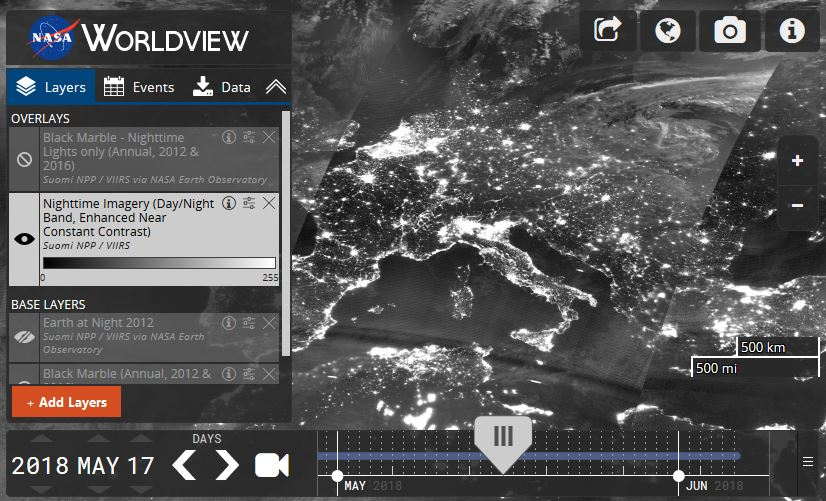
\includegraphics[width=1.0\textwidth]{img/worldview.JPG}
	\caption{Outil de visualisation NASA Worldview \cite{nasa-worldview}.}
	\label{nasa-worldview-screenshot}
\end{figure}

Le premier jeu de données est série d'images composites capturées par le satellite Suomi NPP opéré par la NASA, la NOAA et le Département de la Défense des États-Unis. Il est mis à jour toutes les quelques heures, et présente une image composite chaque jour depuis le 30 novembre 2016. Elle possède deux défauts éliminatoires : la période d'observation actuellement disponible (à peine plus d'une année) n'est pas suffisamment longue pour observer une évolution significative des villes depuis l'espace, et les images ne sont pas traitées. Cela signifie que celles-ci sont très fortement bruitées par les nuages et la lumière ambiante due aux différentes phases de la Lune.

\begin{figure}[h]
	\centering
	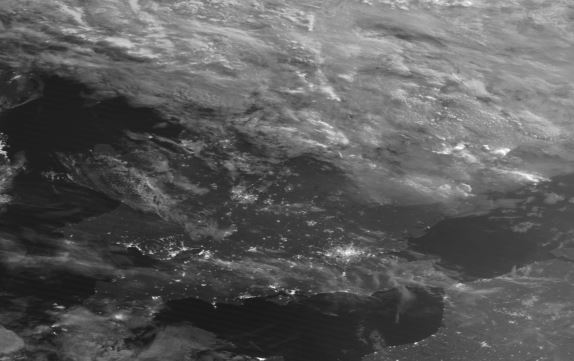
\includegraphics[width=0.5\textwidth]{img/worldview_clouds.JPG}
	\caption{Image satellite quotidienne servie par NASA Worldview \cite{nasa-worldview}, représentant la Grande Bretagne et son climat nuageux.}
	\label{nasa-worldview-daily}
\end{figure}

Les deux autres jeux de données nocturnes sont des images composites : des clichés pris tout au long de l'année ont permis de fabriquer une seule image du globe dont la luminosité ambiante est constante (moyennée) et sur laquelle les nuages n'apparaissent pas. Malheureusement, l'outil Worldview ne permet pas un téléchargement direct de ces images \textit{dans leur pleine résolution}. Heureusement, la NASA a mis à disposition une API REST pour télécharger des "tuiles" de n'importe laquelle de leur image. Seulement le format PNG est disponible. Ce format ne contient pas d'information géographiques, ce qui complique leur utilisation pour la suite de ce travail. Un script Python suffit pour télécharger et assembler les tuiles (figure \ref{nasa-worldview-tile}) pour reconstituer une image complète du globe de plus de 800 millions de pixels (figure \ref{nasa-worldview-tiles}).

\begin{figure}[h]
	\centering
	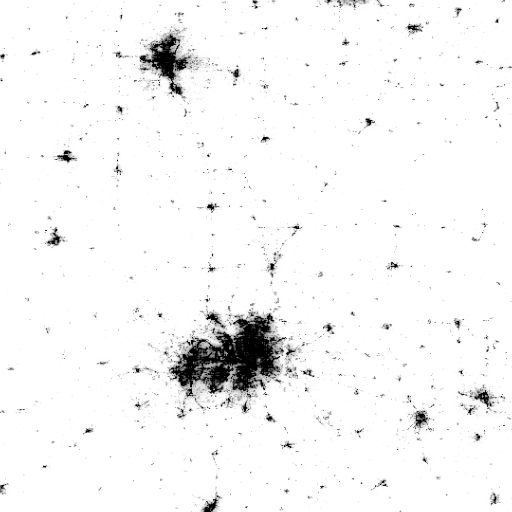
\includegraphics[width=0.5\textwidth]{img/018-012.png}
	\caption{Une tuile de l'image de 2016 \cite{nasa-api} montrant la ville de Dallas (USA) après avoir été mise en couleurs négatives.}
	\label{nasa-worldview-tile}
\end{figure}

\begin{figure}[h]
	\centering
	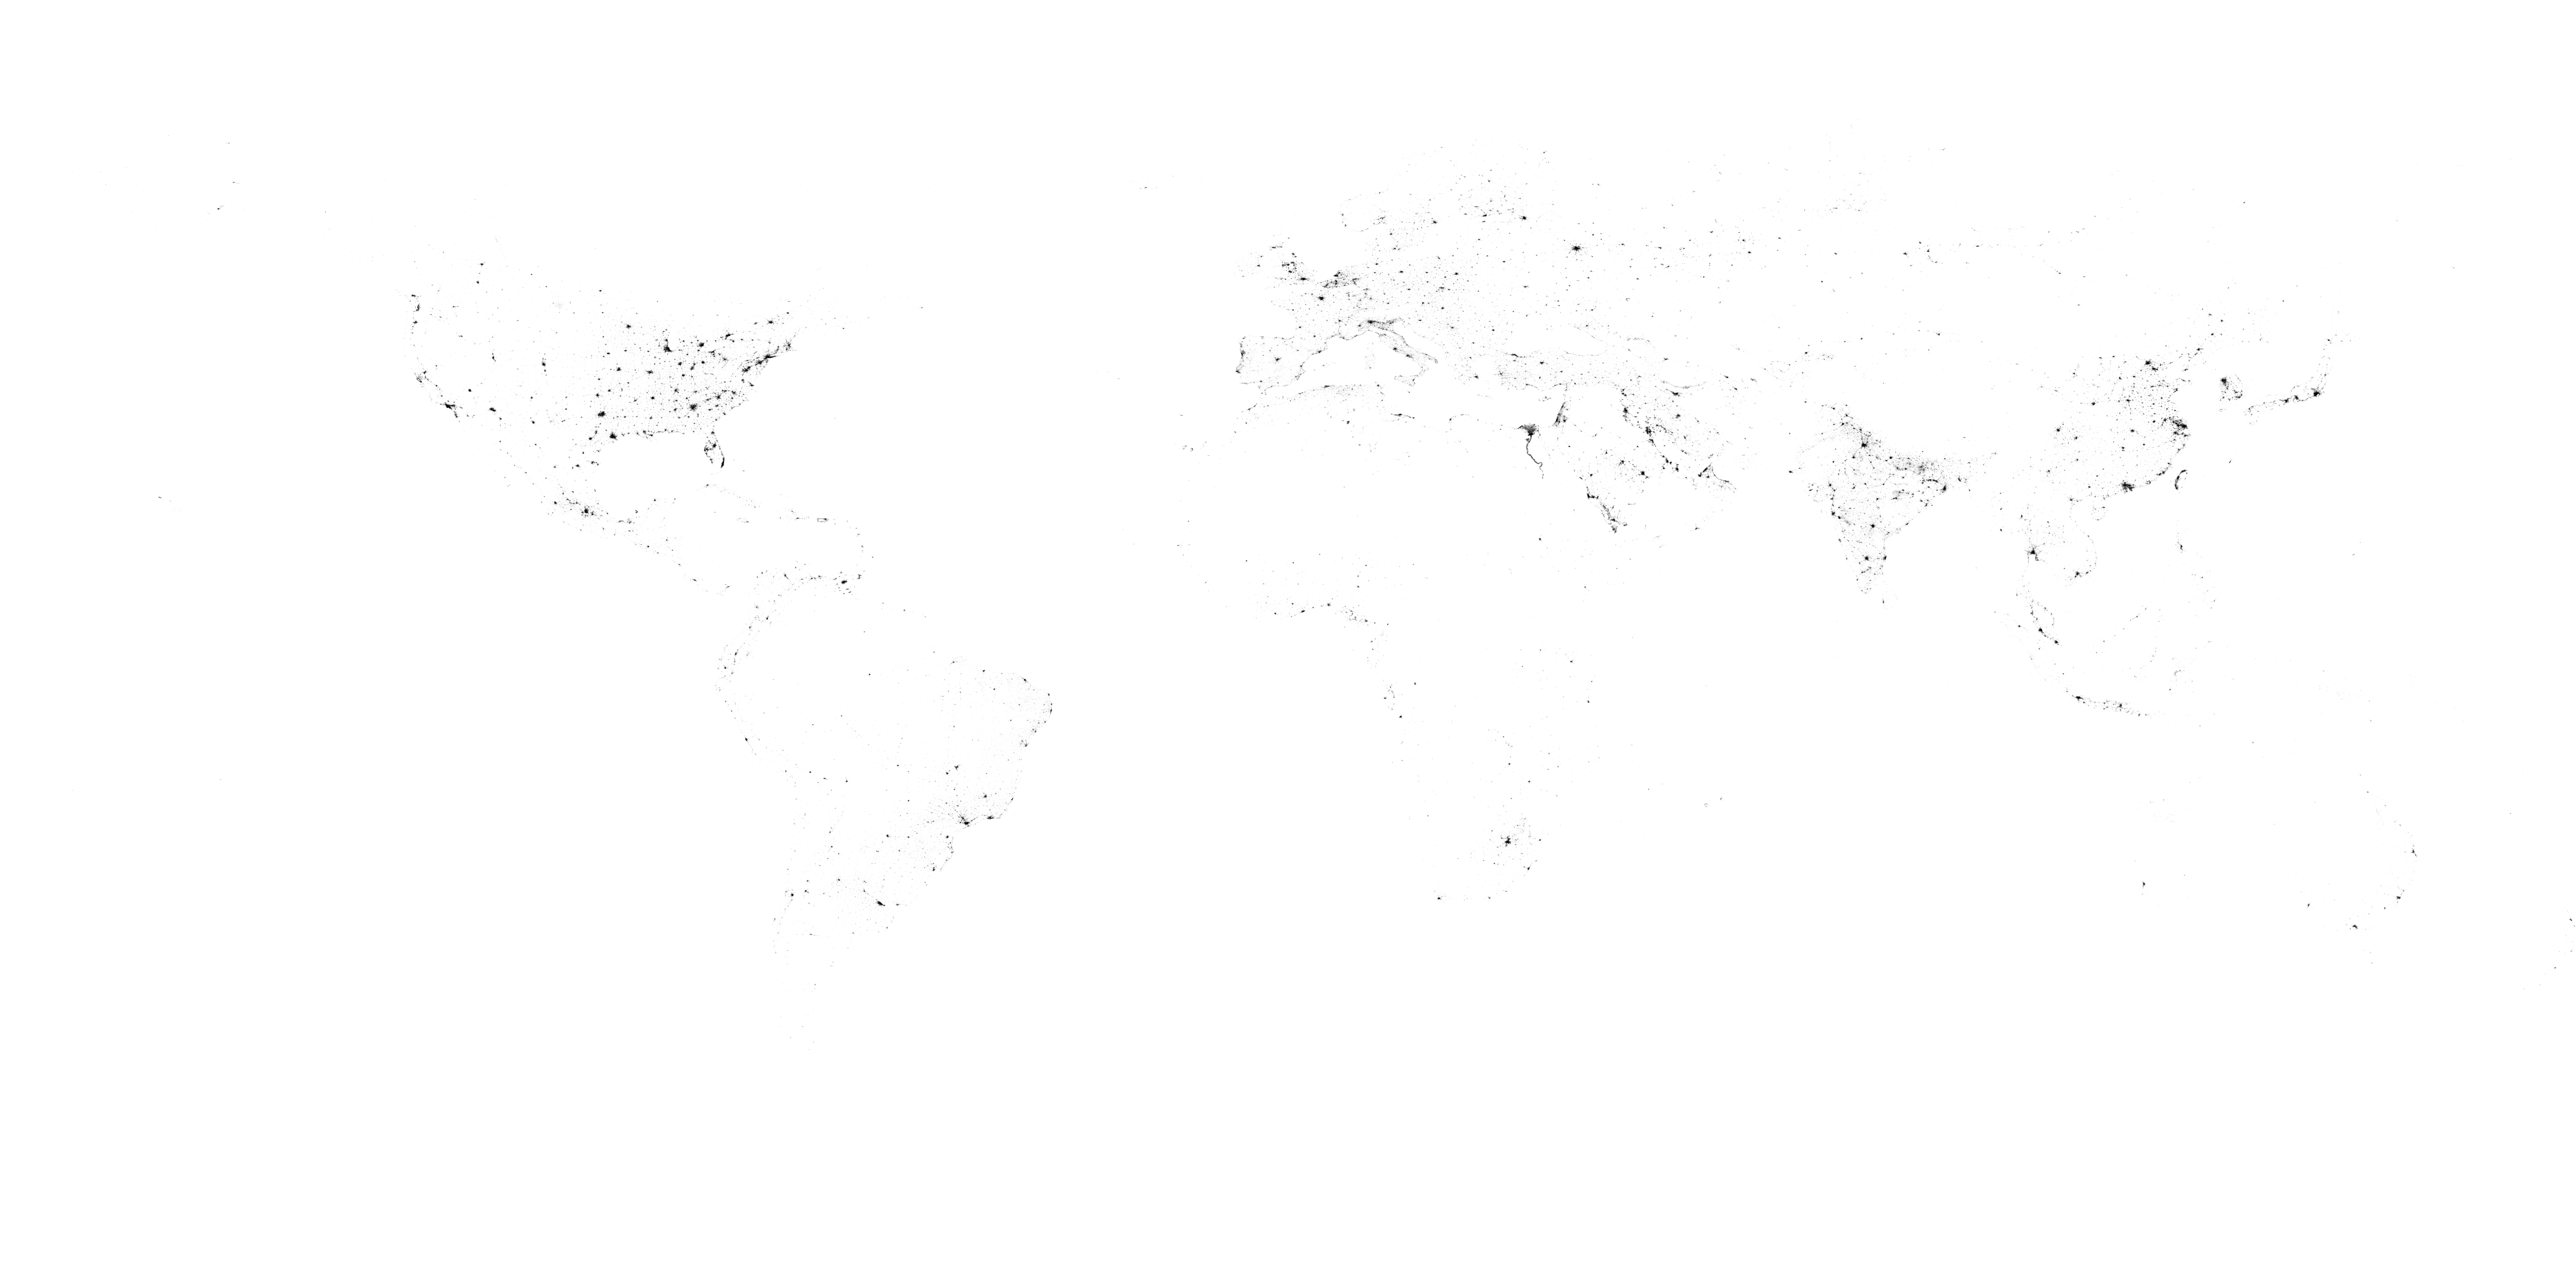
\includegraphics[width=1.0\textwidth]{img/tiles_2016_zoom6.png}
	\caption{Image globale annuelle (2016) reconstituée à partir de tuiles téléchargées \cite{nasa-api}, puis mise en couleurs négatives.}
	\label{nasa-worldview-tiles}
\end{figure}

Le script python utilisé se trouve dans Code/scraper/generate\_all.py et nécessite l'installation de la librarie Pillow pour le traitement des images, ainsi qu'urllib pour le téléchargement en soi. Son exécution peut demander plus d'une heure pour le téléchargement (vitesse limitée par le serveur), et plus de 4 Go de RAM pour l'assemblage des tuiles.

\subsubsection{Agence américaine d'observation océanique et atmosphérique}
La source d'images satellite retenue pour la suite du travail est celle de l'Agence américaine d'observation océanique et atmosphérique (abrégée NOAA)\cite{noaa}. Des images satellites nocturnes composites ("Average Lights X Pct") sont disponibles pour les années 1992 à 2013, une période suffisante pour observer des changements depuis l'espace. De plus, ces données sont disponibles en format GeoTIFF, qui contient les informations géographiques nécessaires pour superposer cette carte à sur autre. Il est donc possible d'explorer et manipuler ces cartes à l'aide de logiciels libres tels que QGIS. Il s'agit en réalité des mêmes clichés fournis par Worldview (et Google Earth), mais plus nombreux et dans un format plus exploitable.

Ces images ont été créées en moyennant la valeur de luminosité de chaque pixel sur une année, en ignorant les pixels couverts par des nuages, et en multipliant cette moyenne par la fréquence de détection de lumière sur le pixel au cours de l'année.

\subsection{Grilles de population}
Sedac \cite{sedac} met à disposition des grilles de populations pour le monde entier, sous forme de fichier GeoTIFF. Chaque "case" de 1 $km^2$ est représentée comme un pixel et contient une estimation du nombre de personnes vivant dans cette case. QGIS s'est à nouveau montré d'une grande aide pour visualiser et manipuler ces données volumineuses (exemple en figure \ref{qgis-sedac}).

On remarque que la valeur de densité de population ne varie pas à l'intérieur d'un sous-région. Tous les pixels d'une grande ville ou d'un département possèdent la même valeur. Ces données ont été créées à partir de plusieurs mesures lorsque le décompte de la population pour une sous-région n'a pas été considéré fiable. Les images satellites font d'ailleurs partie de ces mesures supplémentaires.

Ces cartes sont disponibles pour les années 2000, 2005, 2010, 2015 et 2020.

\begin{figure}[h]
	\centering
	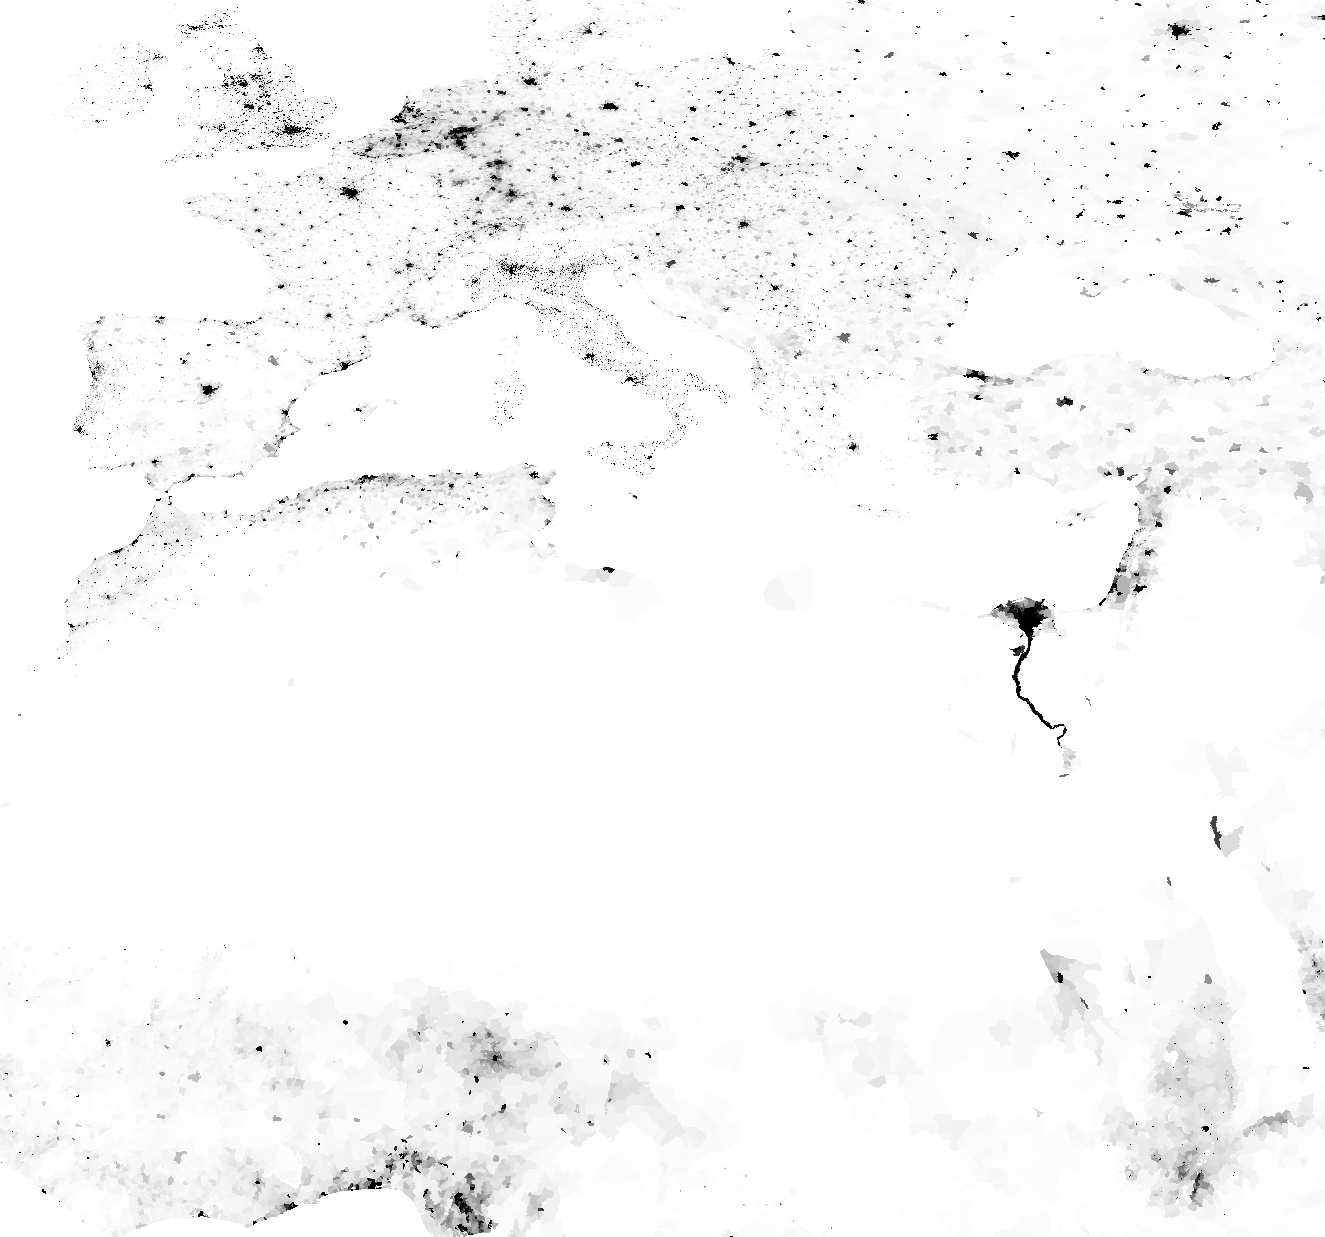
\includegraphics[width=1.0\textwidth]{img/pop_subset.png}
	\caption{Extrait de la grille de population \cite{sedac} rendue par QGIS. Le blanc indique une absence d'habitant, le noir indique plus de 1000 habitants par mètre carré.}
	\label{qgis-sedac}
\end{figure}


\subsection{Pays}
(nightlights, poprasters, vectors, script de download)

\section{Recherche de corrélation}
Recherche de corrélation, graphes

Problème de format pour la superposition des rasters


GPD, groupement par pays, filtré par développement économique, graphes

deltas de luminosité par pays, incomplet

\section{Données à explorer}
Données encore pas explorées : human footprint, ...

\chapter{Modèle neuronal}
\section{Réseau de neurones}
réseau de neurones à convolution pour faire de la régression => chercher des cas de peoblèmes similaires

\section{Environnement de développement}
installation : keras, tensorflow, setup nvidia

\section{Métaparamètres}
métaparamètres du réseau de neurones

\chapter{Conclusion}
Travail effectué, travail restant

\printbibliography

\chapter{Authentification}


\chapter{Symboles et abréviations}


\listoffigures

\chapter{Annexes}

\end{document}